\section{Use-Case}
\label{sect:useCase}

This section describes an usecase to demonstrate the cit-storm framework. Each operator listed in the second section is provide by the cit-storm framework and can be combined with each other to form a meaningfull topology. In this work we analyze the twitter stream in a real-time fashion to find significant users and if once detected all following tweets are stored in a cassandra database. Tweets are split up into single words and only words from an internal badwords-table filtered to computate a user-tweet significance and finally added to a total user-significance. \newline

Figure 1 shows the final topology which uses the most of all operators. The Topology consists of two different data streams originatd at the twitter streaming source. The upper stream is responsible to keep a tweet inside the network as long as the tweet is analyzed, what is realized by an delayed-operator. The stream on the bottom analyze the tweets by linking different operators to each other. The first flatmap operator splits each tweet into single words and join these with an internal hashmap to filter only words which belongs to a word-list of interest.


\begin{figure}[h]
  \centering
  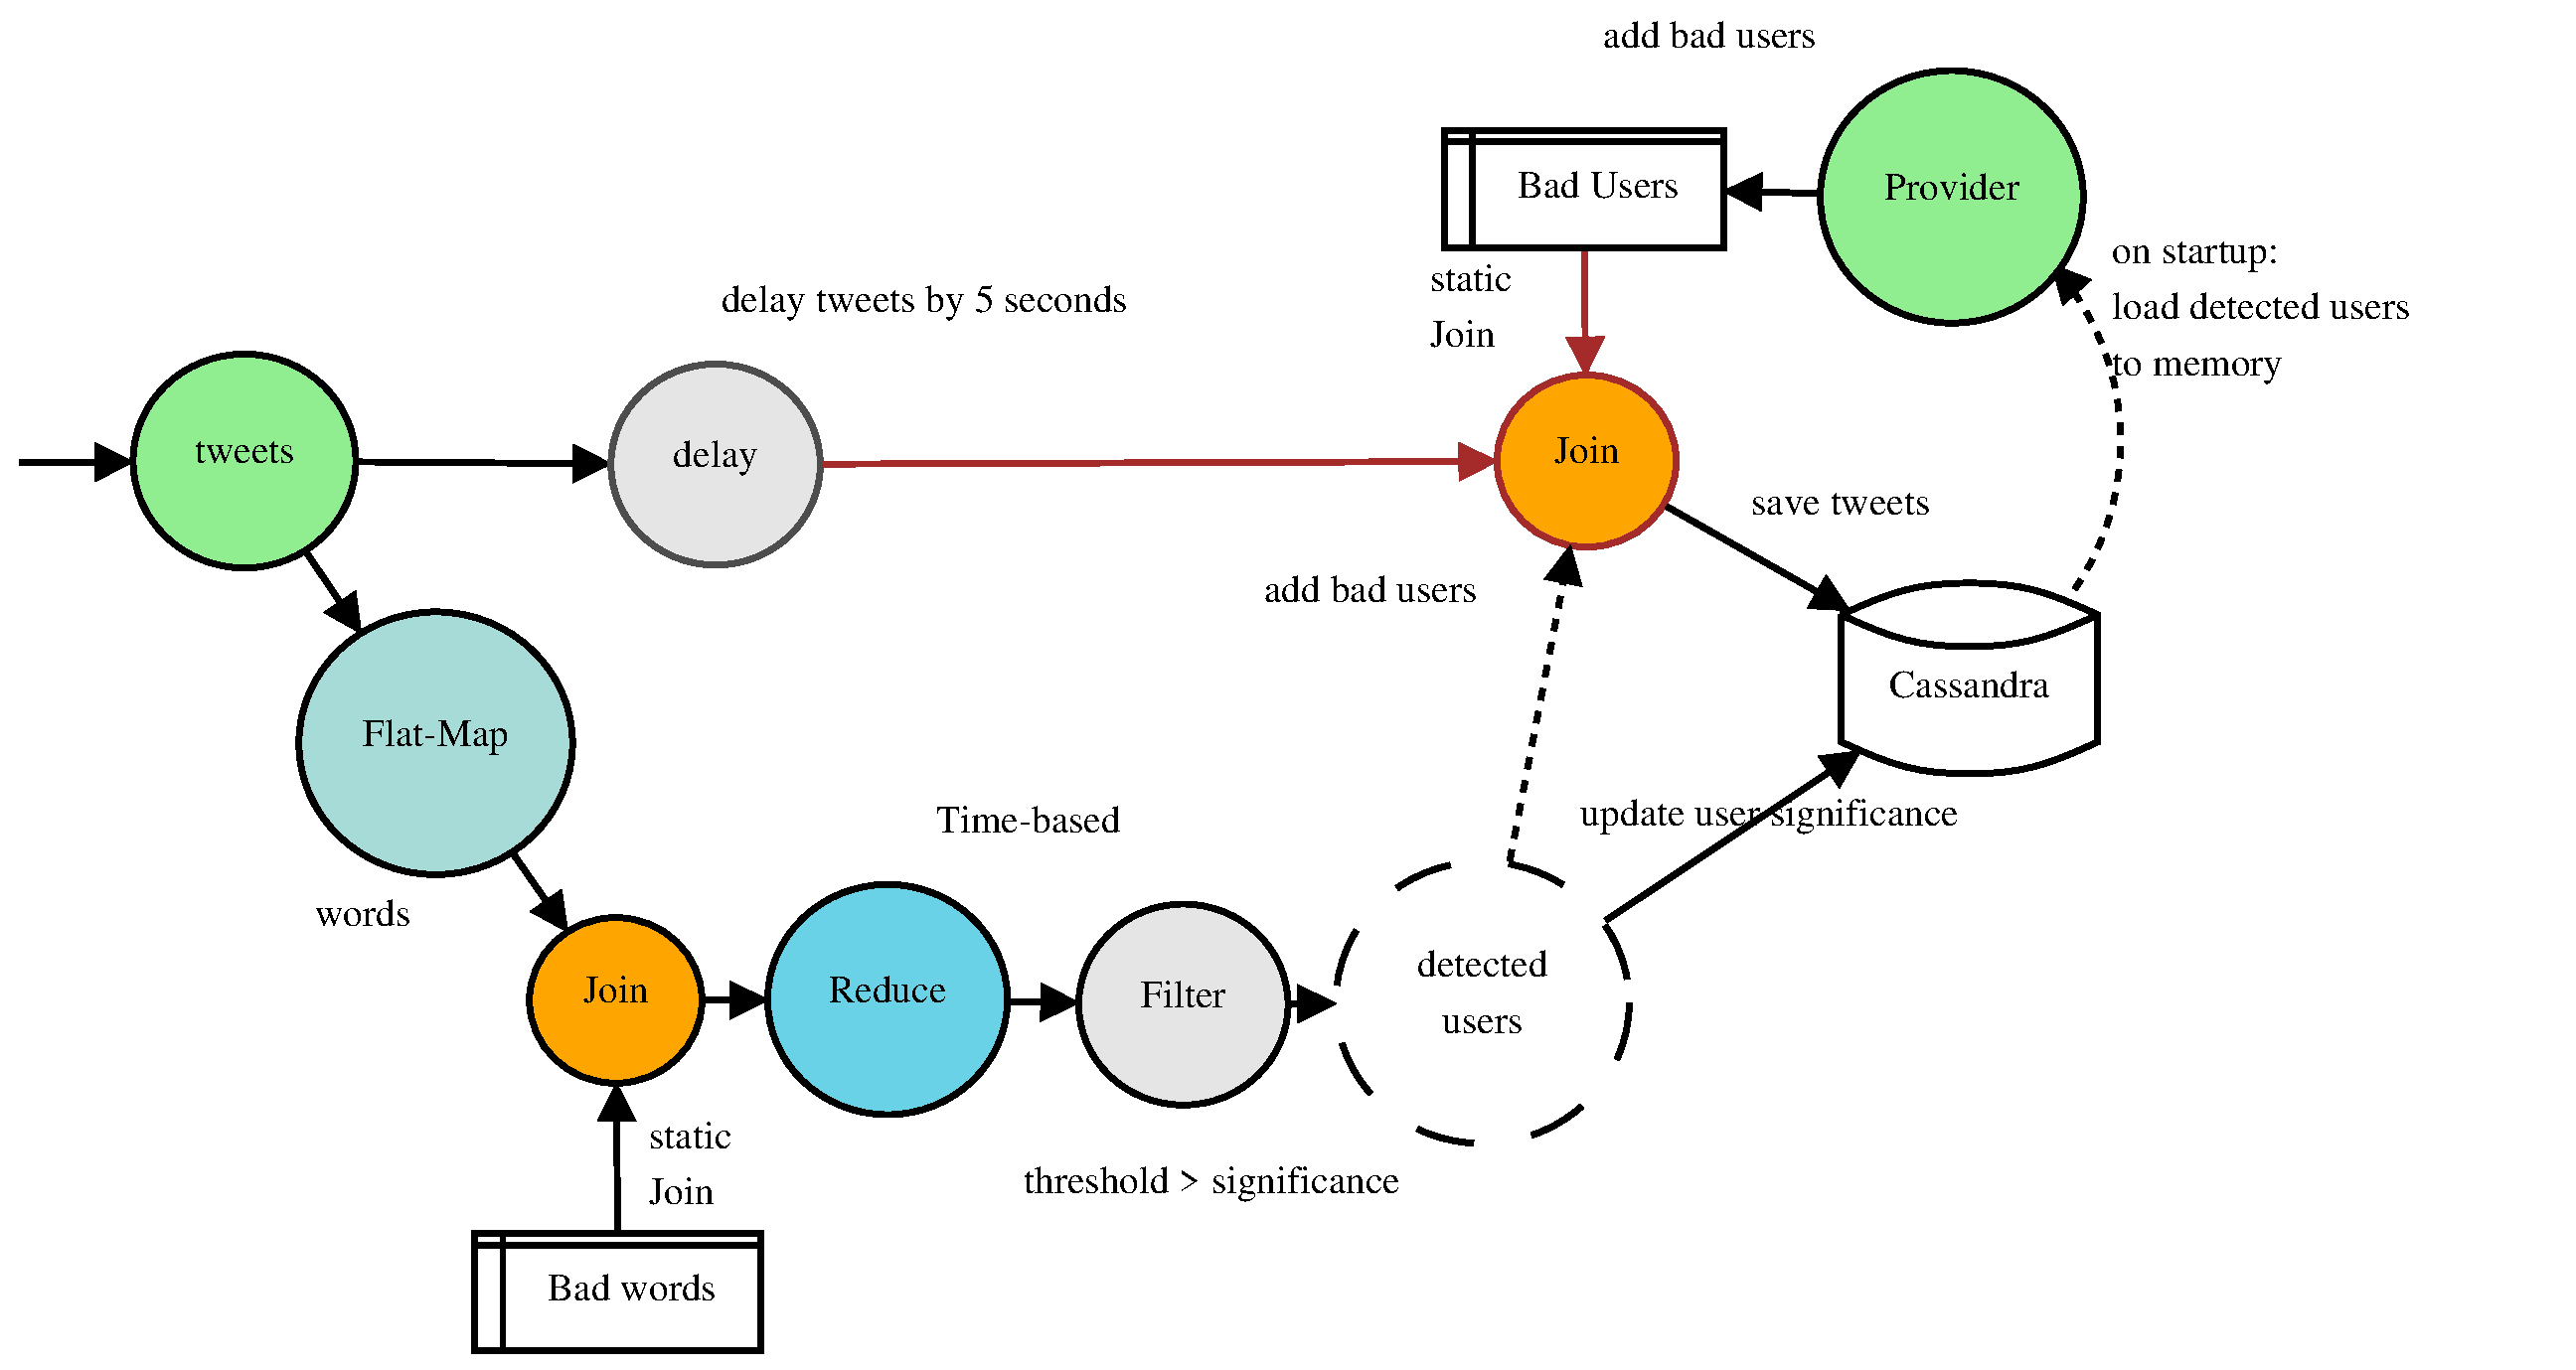
\includegraphics[width=0.5\textwidth]{images/AnalyzeTweetsTopology}
  \caption{This figure shows all operators used in the topology and how they are realted to each other. Operators are depicted as filled circles, in-memory storage is depicted as rectangles and dotted circles describe outputs within a operator for clarification. }
           
\end{figure}
